\chapter{Specific Requirements}

\section{External Interface Requirements}
\subsection{User Interface}
This section presents mockups of the most relevant graphical user interfaces (GUIs) used by the 
Student\&Companies platform to interact with external users, such as companies' employees and students. 
The purpose of these representations is to outline the 
logical characteristics of the interfaces and provide guidelines on the style and appearance of the final product. 

\paragraph{Log In Interface}
Log In Interface for both Companies and Students, 
username, email and password are required. 
Once every field is filled correctly the user can access 
pressing the Log In button.
\begin{figure} [H]
    \centering
    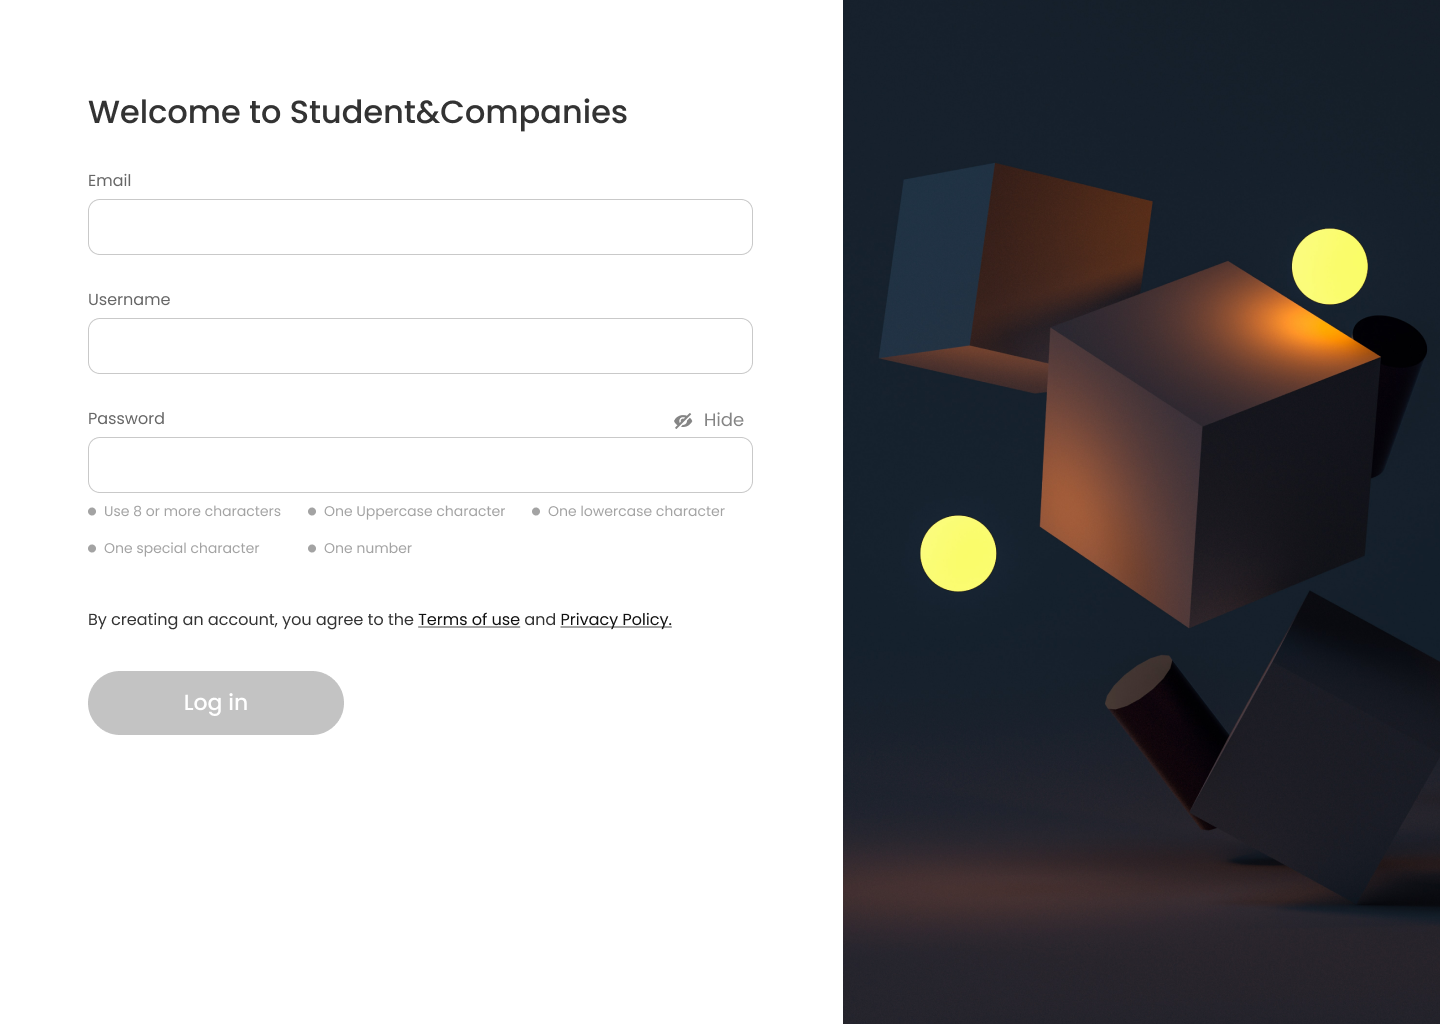
\includegraphics [width=.7\linewidth] {login.png}
\end{figure}

\paragraph{Available Intership List}
This inteface displays the available internships, the
view is optimized based on the Recommendation Engine.
\begin{figure} [H]
    \centering
    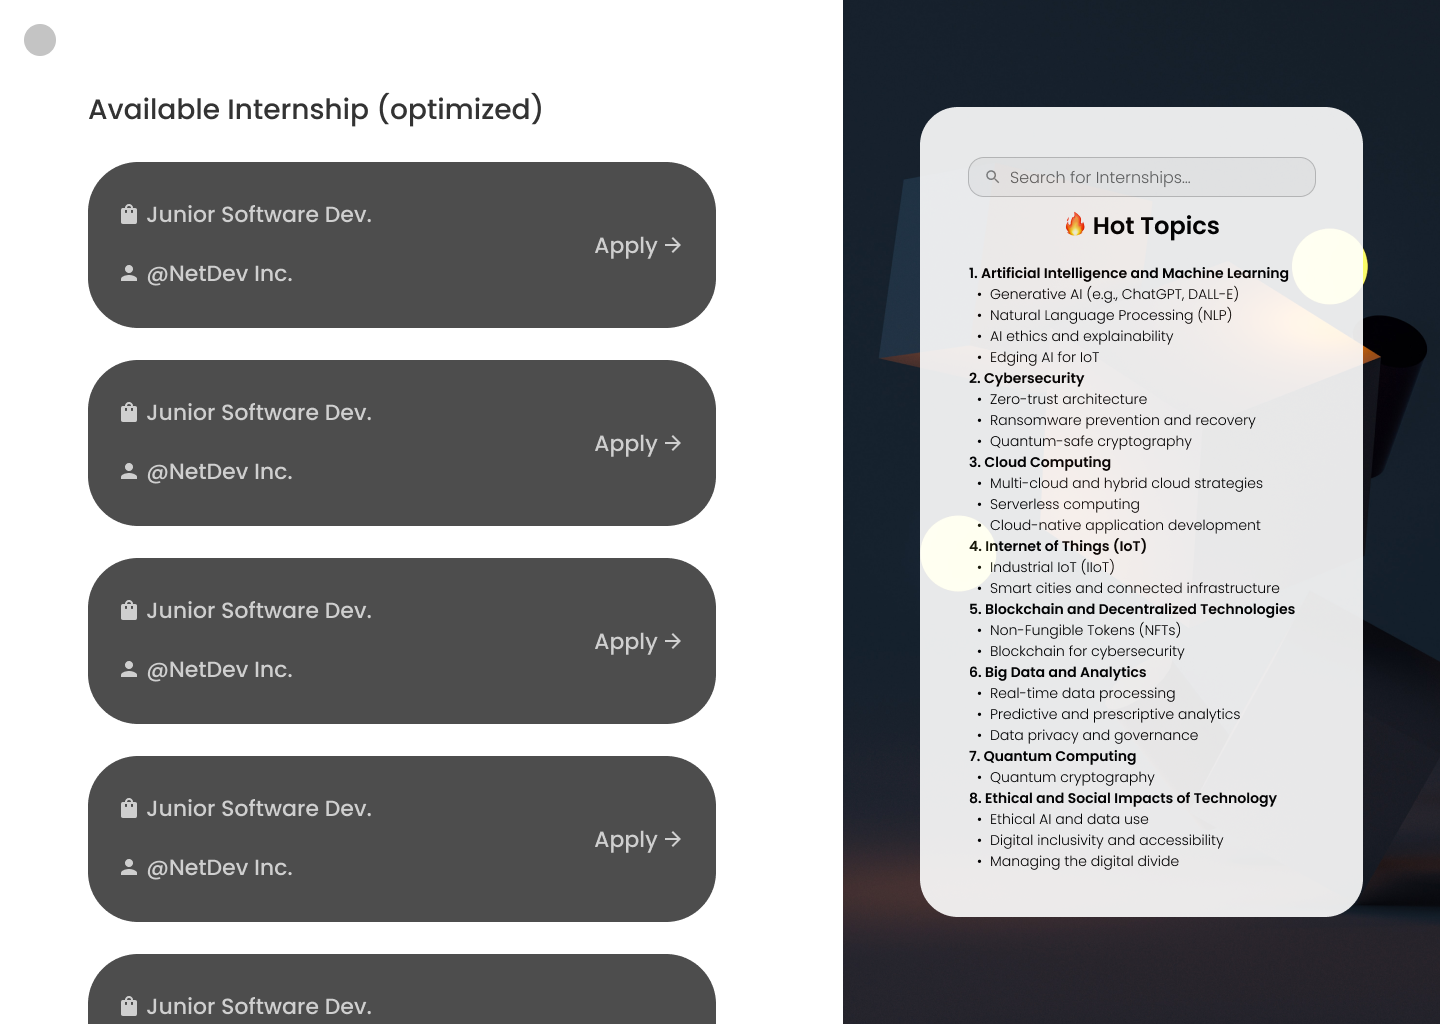
\includegraphics [width=.7\linewidth] {internshipBrowsing.png}
\end{figure}

\paragraph{Student and Company Profile View}
Both Students and Companies pages have a profile picture of their choice,
an email and a phone number as contact information,
however they differ slightly, 
as the Student has the university in which he/she belongs
displayed at the bottom, while the Company has the the name
of the current CEO.
Furthermore, on the left, the Student page allows anyone
to download the Student's CV, whereas the Company's page
displays its available internships.
\begin{figure} [H]
    \centering
    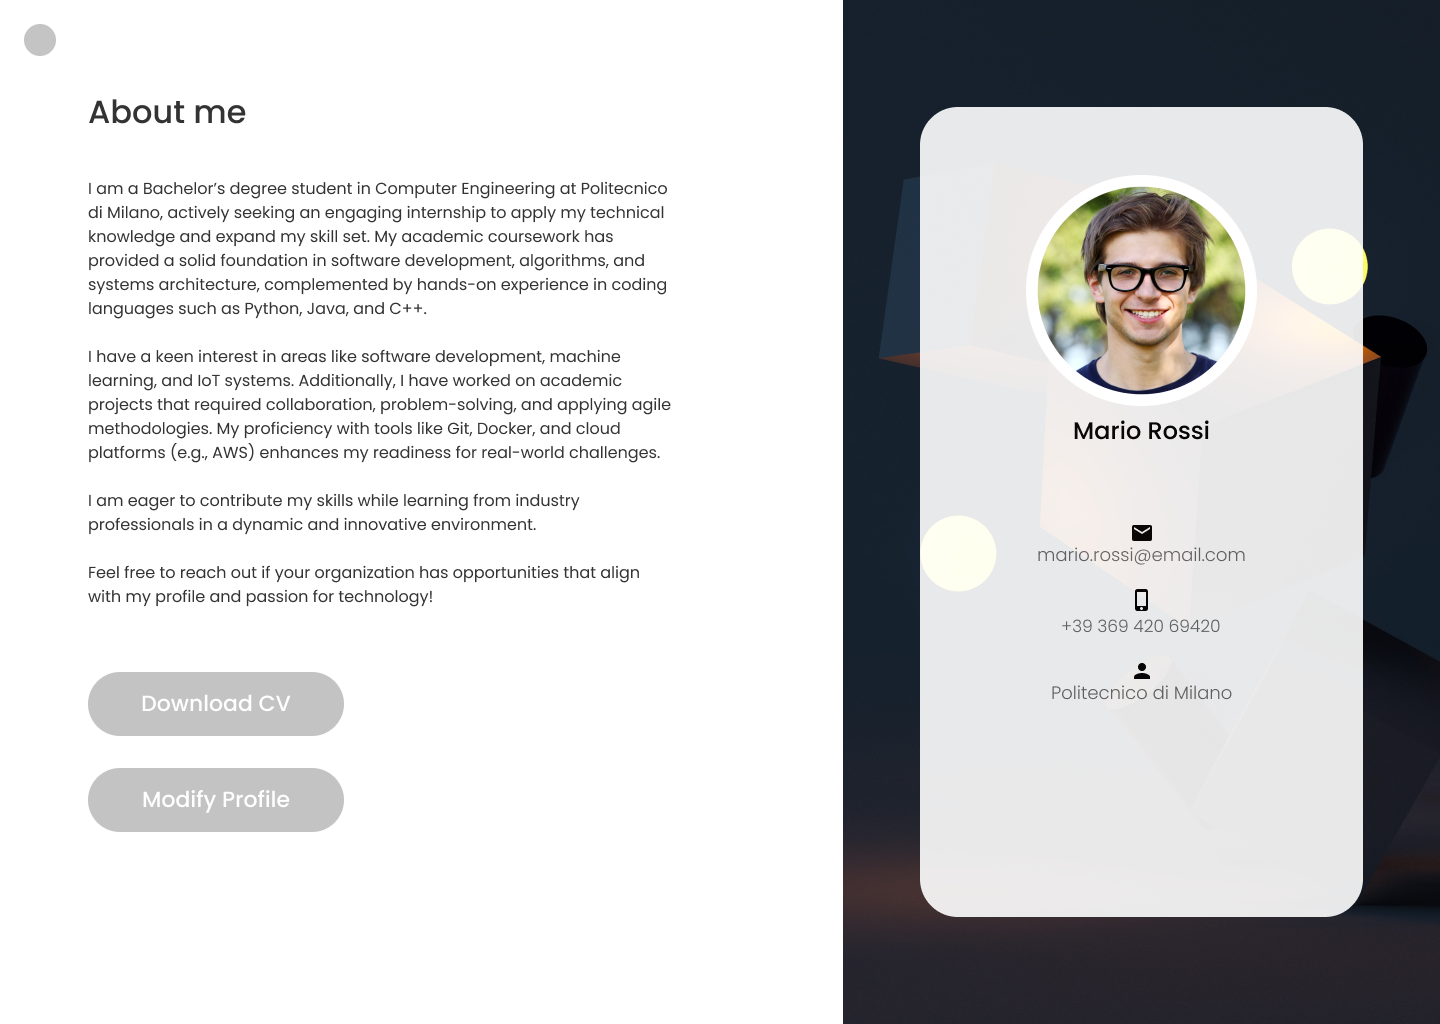
\includegraphics [width=.7\linewidth] {studentProfile.png}
\end{figure}
\begin{figure} [H]
    \centering
    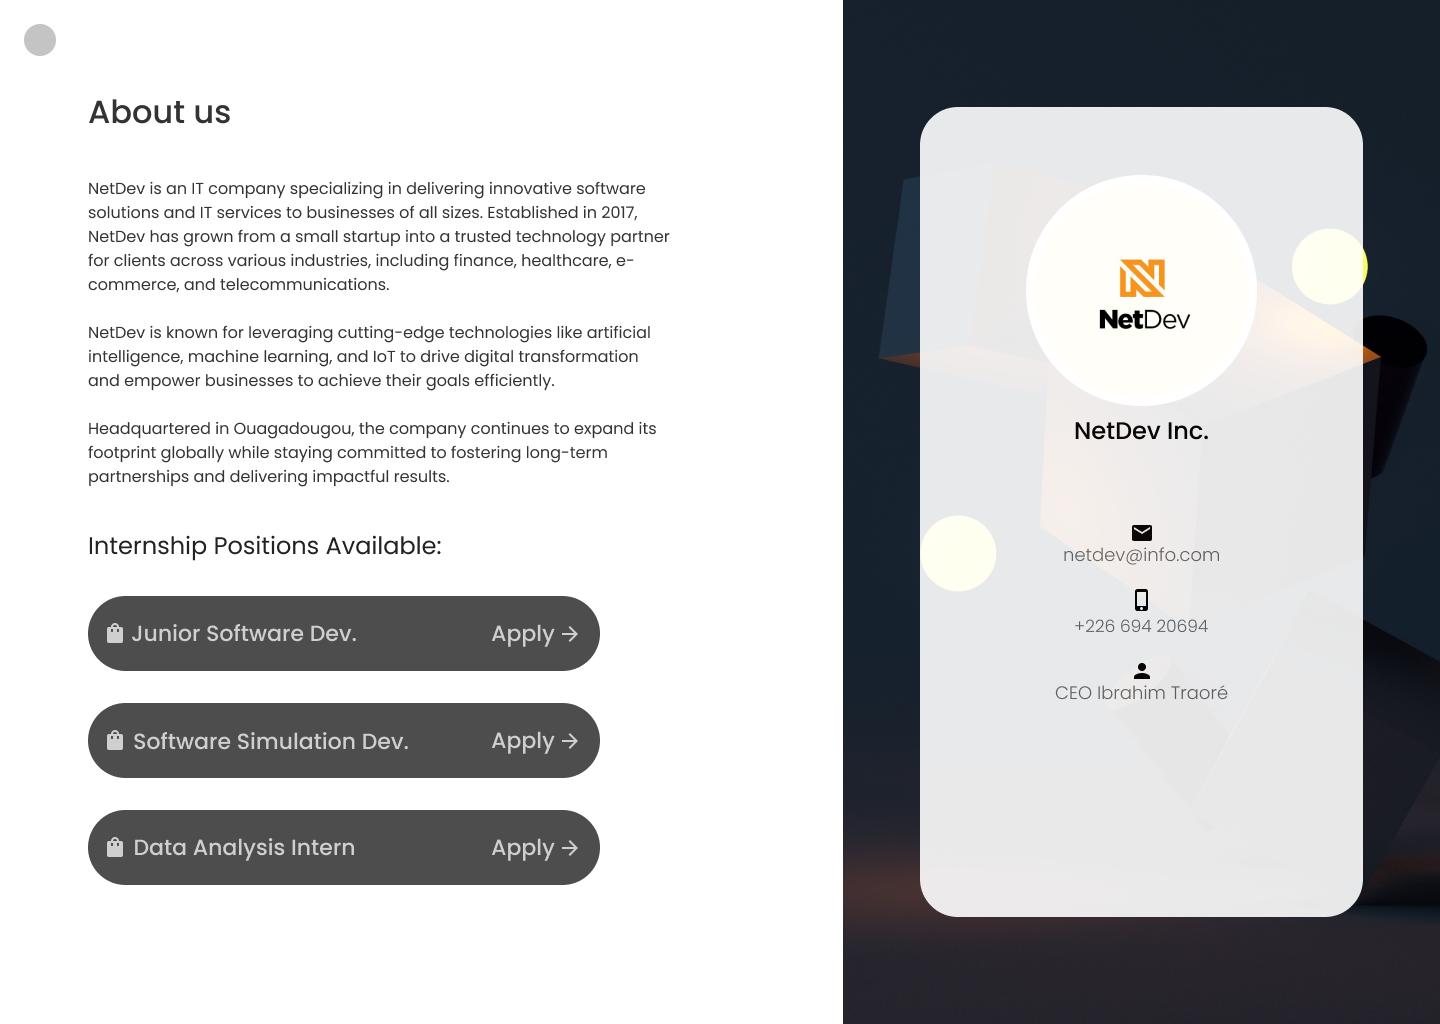
\includegraphics [width=.7\linewidth] {companyProfile.png}
\end{figure}

\paragraph{Internship Creation Form and Preliminary Internship Questionnaire}
Both interfaces are forms with different purposes, the first is
exclusively for Companies, mandatory in order to create a new intership
position which will be available for Students' application.
The second is exclusively for Students, this form will appear after 
a Student click apply on an available internship.
\begin{figure} [H]
    \centering
    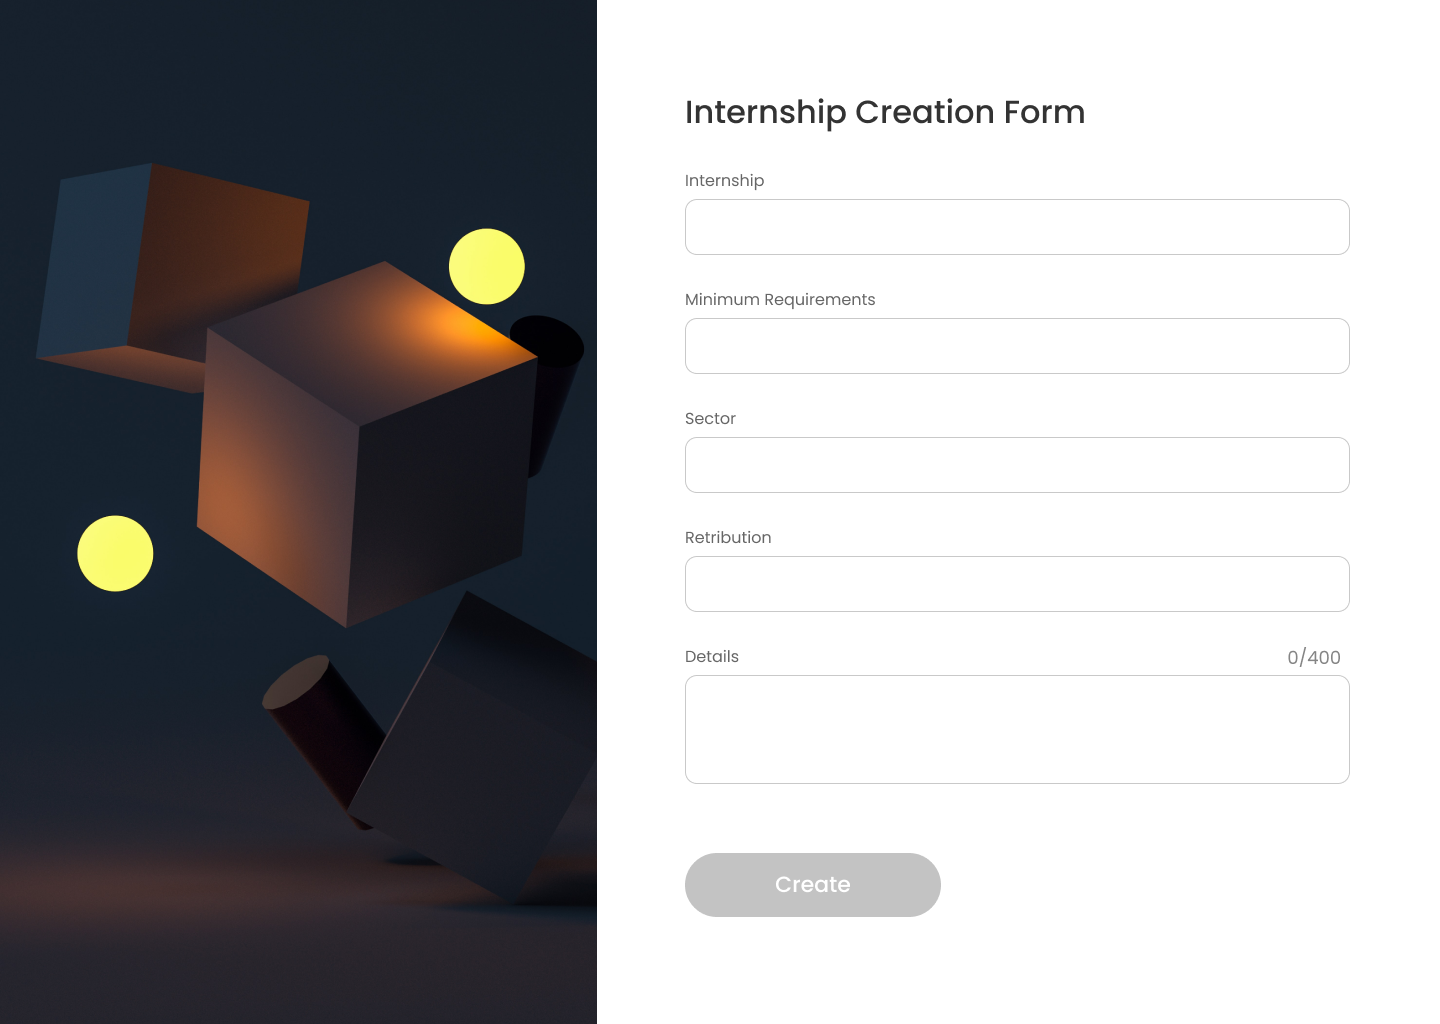
\includegraphics [width=.7\linewidth] {internshipCreationForm.png}
\end{figure}
\begin{figure} [H]
    \centering
    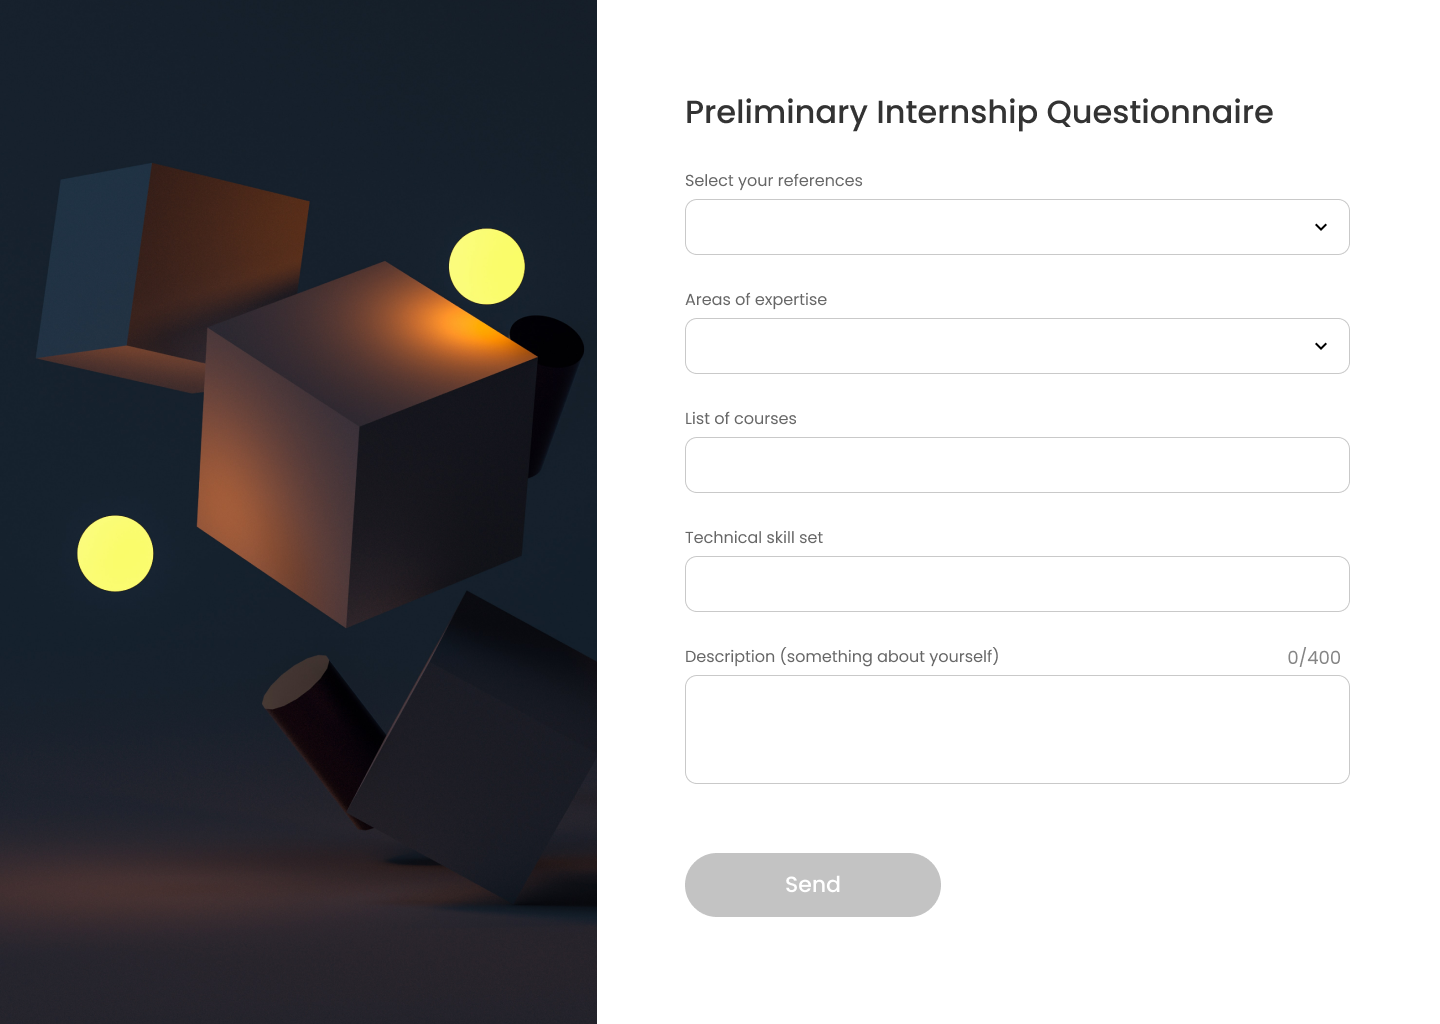
\includegraphics [width=.7\linewidth] {questionnaire.png}
\end{figure}

\subsection{Hardware Interface}
The S\&C platform requires a server to host all its 
functionalities, in order to offer the best service possible
the server machine requires some key hardware components with 
their corresponding interfaces:

\begin{itemize}
    \item A processor (CPU) capable of handling concurrent user requests and process data.
    \item Main memory (RAM).
    \item Data Storage (Hard Disk/SSD).
    \item  Network Interface Card (NIC): A reliable network interface for communication
    between the server and users’ devices.
\end{itemize}

S\&C will be an online web platform so the following hardware 
components are also mandatory:

\begin {itemize}
    \item High speed and reliable Internt Connection in order to maintain a running platform and guarantee efficiency
    \item Firewall and Security Protocols for the safety of users data
    \item Load Balancers
\end {itemize}

The end-users' minimus requirements (hardware wise) are:

\begin {itemize}
    \item Computer or Mobile devices
    \item Reliable Internet connection
    \item Network Interface Card
\end {itemize}

\subsection{Software Interface}
\begin {itemize}
    \item Client-server interactions occur by the means of a HTTPS protocol to exchange data and information
    \item Database Interface as a database is needed to store and manipulate users' data
\end {itemize}

\section{Functional Requirements}
\subsection{Use Case Diagram}
\begin{figure} [H]
    \centering
    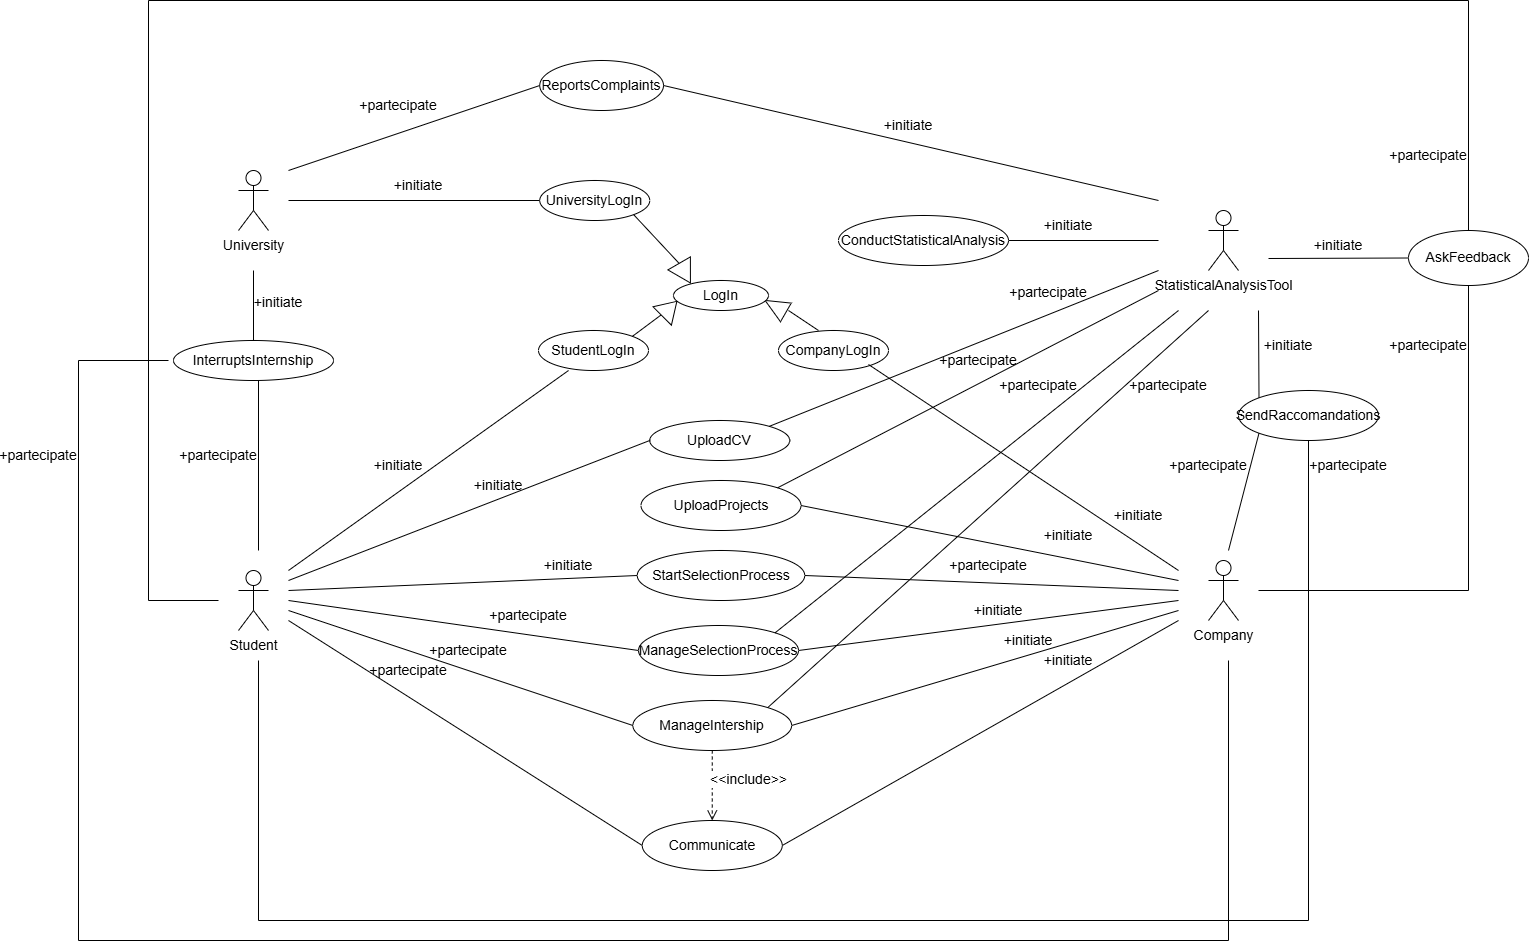
\includegraphics [width=.8\linewidth] {usecasewhite.png}
    \caption{S\&C Use Case Diagram}
\end{figure}
A UML Use Case Diagram visually represents the interactions between users (actors) and the system. 
It focuses on identifying the system's functionalities (use cases) and how various actors engage with them.
These diagrams are essential for understanding system requirements, defining its scope, and providing a high-level overview of user-system interactions, 
making them particularly useful in requirement analysis.
The diagram identifies key actors such as Students, Companies, Universities, and the Statistical Analysis Tool (internal to the platform) 
and captures their interactions with the system's core processes. Key use cases include:

\begin{itemize}
\item Searching and Applying for Internships:
Students can proactively search through available internships and apply to those matching their skills and interests.

\item Publishing Internship Offers:
Companies can advertise internships, providing detailed descriptions, requirements, and terms.

\item Recommendation Mechanism:
The system matches students with suitable internships based on keyword searches, statistical analysis, and feedback data.

\item Selection and Interview Management:
Companies use the platform to manage interviews and assess candidates through questionnaires.

\item Feedback and Complaints:
Both students and companies provide feedback, which is used to improve the recommendation process and refine submissions (e.g., CVs or project descriptions).

\item Monitoring and Issue Handling
Universities, monitor internships, address complaints, and ensure proper resolution of disputes.
\end {itemize}

\subsection{Use Cases}
This section outlines the primary interactions between users and the system, 
detailing the various scenarios in which the system is utilized to achieve specific goals. 
Each use case describes the roles of actors, the sequence of actions, and the expected outcomes, 
providing a clear understanding of how the system fulfills its functional requirements. 

\begin{table}[H]
    \centering
    \renewcommand{\arraystretch}{2}
    \begin{tabular}{|l|p{10cm}|}
    \hline
    \textbf{Use Case ID} & [UC1] - StudentLogsIn \\ \hline
    \textbf{Name} & StudentLogIn \\ \hline
    \textbf{Actors} & Student \\ \hline
    \textbf{Entry Condition} & Student has opened the S\&C application. \\ \hline
    \textbf{Event Flow} & 
    1. S\&C shows the log in interface. \newline
    2. Student clicks on the button to sign in. \newline
    3. Student is redirected to their university's login page. \newline
    4. Student inserts his/her credentials and confirms. \\ \hline
    \textbf{Exit Condition} & S\&C shows the initial (home) page of the application for a student. \\ \hline
    \textbf{Exceptions} & 
    1. If the student inserts incorrect credentials, the authentication page will return an error and ask him/her to retry. \\ \hline
    \end{tabular}
\end{table}

\newpage

\begin{table}[H]
    \centering
    \renewcommand{\arraystretch}{2}
    \begin{tabular}{|l|p{10cm}|}
    \hline
    \textbf{Use Case ID} & [UC2] - CompanyLogsIn \\ \hline
    \textbf{Name} & CompanyLogIn \\ \hline
    \textbf{Actors} & Company \\ \hline
    \textbf{Entry Condition} & Company has opened the S\&C application. \\ \hline
    \textbf{Event Flow} & 
    1. S\&C shows the log in interface. \newline
    2. Company clicks on the button to sign in. \newline
    3. Company is redirected to its login page. \newline
    4. Company inserts his/her credentials and confirms. \\ \hline
    \textbf{Exit Condition} & S\&C shows the initial (home) page of the application for a company. \\ \hline
    \textbf{Exceptions} & 
    1. If the company inserts incorrect credentials, the authentication page will return an error and ask him/her to retry. \\ \hline
    \end{tabular}
\end{table}

\newpage

\begin{table}[H]
    \centering
    \renewcommand{\arraystretch}{2}
    \begin{tabular}{|l|p{10cm}|}
    \hline
    \textbf{Use Case ID} & [UC3] - UniversityLogIn \\ \hline
    \textbf{Name} & UniversityLogIn \\ \hline
    \textbf{Actors} & University \\ \hline
    \textbf{Entry Condition} & University has opened the S\&C application. \\ \hline
    \textbf{Event Flow} & 
    1. S\&C shows the log in interface. \newline
    2. University clicks on the button to sign in. \newline
    3. University is redirected to their login page. \newline
    4. University inserts his/her credentials and confirms. \\ \hline
    \textbf{Exit Condition} & S\&C shows the initial (home) page of the application for a university. \\ \hline
    \textbf{Exceptions} & 
    1. If the university inserts incorrect credentials, the authentication page will return an error and ask him/her to retry. \\ \hline
    \end{tabular}
\end{table}

\newpage
    
\begin{table}[H]
    \centering
    \renewcommand{\arraystretch}{2}
    \begin{tabular}{|l|p{10cm}|}
    \hline
    \textbf{Use Case ID} & [UC4] - UploadCV \\ \hline
    \textbf{Name} & UploadCV \\ \hline
    \textbf{Actors} & Student, StatisticalAnalysisTool \\ \hline
    \textbf{Entry Condition} & Student is logged in to the S\&C platform. \\ \hline
    \textbf{Event Flow} & 
    1. Student clicks on the button to modify his/her profile. \newline
    2. S\&C shows the form to fill with the information for the profile to be modified, including the space to upload the CV. \newline
    3. Student modifies his/her profile. \newline
    4. Student uploads his/her CV. \newline
    5. Student confirms the changes. \newline
    6. S\&C applies the changes. \newline
    7. StatisticalAnalysisTool collects data regarding the student's profile. \\ \hline
    \textbf{Exit Condition} & The student's profile is modified. \\ \hline
    \textbf{Exceptions} & 
    1. The CV is not in one of the supported formats. S\&C returns an error message indicating the correct formats. \newline
    2. One of the mandatory fields has not been filled. S\&C returns an error message indicating the mandatory fields. \\ \hline
    \end{tabular}

\end{table}

\newpage
    
\begin{table}[H]
    \centering
    \renewcommand{\arraystretch}{2}
    \begin{tabular}{|l|p{10cm}|}
    \hline
    \textbf{Use Case ID} & [UC5] - UploadProjects \\ \hline
    \textbf{Name} & UploadProjects \\ \hline
    \textbf{Actors} & Company, StatisticalAnalysisTool \\ \hline
    \textbf{Entry Condition} & Company is logged in to the S\&C platform. \\ \hline
    \textbf{Event Flow} & 
    1. Company clicks on the button to create a new project. \newline
    2. S\&C shows the form to fill with the information about the new project. \newline
    3. Company fills out the form. \newline
    4. Company confirms the details. \newline
    5. S\&C creates a new page dedicated to the project. \newline
    6. StatisticalAnalysisTool collects data regarding the company's project. \\ \hline
    \textbf{Exit Condition} & The page dedicated to the company's project is created. \\ \hline
    \textbf{Exceptions} & 
    1. One of the mandatory fields has not been filled. S\&C returns an error message indicating the mandatory fields. \newline
    2. One of the documents to upload is not in one of the supported formats. S\&C returns an error message indicating the correct formats. \\ \hline
    \end{tabular}
\end{table}

\newpage
    
\begin{table}[H]
    \centering
    \renewcommand{\arraystretch}{2}
    \begin{tabular}{|l|p{10cm}|}
    \hline
    \textbf{Use Case ID} & [UC6] - StartSelectionProcess \\ \hline
    \textbf{Name} & StartSelectionProcess \\ \hline
    \textbf{Actors} & Student, Company \\ \hline
    \textbf{Entry Condition} & Student is logged in to the S\&C platform, and the page dedicated to the project has been created. \\ \hline
    \textbf{Event Flow} & 
    1. Student visits the page dedicated to the project. \newline
    2. Student clicks on the button to ask to start the selection process. \newline
    3. S\&C notifies the company about the student's request. \newline
    4. Company visits the profile of the student to check if he/she meets the project's requirements. \newline
    5. Company downloads the student's CV to check if he/she meets the project's requirements. \newline
    6. Company visits the page of the requests for its project. \newline
    7. Company accepts the student for the selection process. \newline
    8. S\&C establishes a contact between the student and company. \\ \hline
    \textbf{Exit Condition} & The selection process has started, and a contact has been established between the student and the company. \\ \hline
    \textbf{Exceptions} & 
    1. The student tries to apply for an internship for which the time window available for requests has ended. S\&C displays an error message informing the student that the time window has closed. \newline
    2. The student tries to apply for an internship for which all places have already been assigned. S\&C displays an error message informing the student that the places have been filled. \\ \hline
    \end{tabular}
\end{table}

\newpage
    
\begin{table}[H]
    \centering
    \renewcommand{\arraystretch}{2}
    \begin{tabular}{|l|p{10cm}|}
    \hline
    \textbf{Use Case ID} & [UC7] - ManageSelectionProcess \\ \hline
    \textbf{Name} & ManageSelectionProcess \\ \hline
    \textbf{Actors} & Student, Company, StatisticalAnalysisTool \\ \hline
    \textbf{Entry Condition} & The selection process of the student has started. \\ \hline
    \textbf{Event Flow} & 
    1. Company clicks the button to allow the student to fill the preliminary questionnaire. \newline
    2. S\&C notifies the student that he/she can fill the preliminary questionnaire. \newline
    3. Student fills the preliminary questionnaire. \newline
    4. S\&C notifies the company that the student has filled the questionnaire. \newline
    5. Company fills out a form regarding the progress of the preliminary questionnaire in the dedicated private space provided by the platform. \newline
    6. StatisticalAnalysisTool collects data about the first part of the selection process. \newline
    7. Company asks the student to participate in an interview. \newline
    8. S\&C notifies the student that he/she has been invited to participate in an online interview. \newline
    9. Student accepts the invitation. \newline
    10. Company interviews the student. \newline
    11. Company fills out a form regarding the progress of the interview in the dedicated private space provided by the platform. \newline
    12. Company finalizes the selection of the candidate student for the internship. \newline
    13. StatisticalAnalysisTool collects data about the selection process. \\ \hline
    \textbf{Exit Condition} & The selection process is over, and the student has been selected by the company for the internship. \\ \hline
    \textbf{Exceptions} & 
    1. The student tries to participate in the online interview on a different date and/or time than the pre-established ones. S\&C displays an error message indicating the correct date and time. \\ \hline
    \end{tabular}
\end{table}

\newpage
    
\begin{table}[H]
    \centering
    \renewcommand{\arraystretch}{2}
    \begin{tabular}{|l|p{10cm}|}
    \hline
    \textbf{Use Case ID} & [UC8] - ManageInternship \\ \hline
    \textbf{Name} & ManageInternship \\ \hline
    \textbf{Actors} & Student, Company, StatisticalAnalysisTool \\ \hline
    \textbf{Entry Condition} & Student has been selected by the company for the internship. \\ \hline
    \textbf{Event Flow} & 
    1. Company finalizes the selection of the candidate student for the internship. \newline
    2. S\&C creates a page dedicated to the specific internship of the specific student for official announcements. \newline
    3. S\&C opens the communication channel. \newline
    4. S\&C notifies the student that the communication channel is opened. \newline
    5. S\&C notifies the company that the communication channel is opened. \newline
    6. Company writes in the dedicated space information about the beginning of the internship. \newline
    7. S\&C notifies the student about the publication of information about the internship. \newline
    8. Student and company communicate through the communication channel (see UC11). \newline
    9. Company publishes information about the current status of the ongoing situation in the dedicated space. \newline
    10. Student writes comments in the dedicated space. \newline
    11. S\&C notifies the student about the new publication. \newline
    12. At the end of the pre-established period of the internship, the company confirms the end of the internship through the dedicated space. \newline
    13. S\&C notifies the student that the internship is over. \newline
    14. S\&C notifies the company that the internship is over. \newline
    15. S\&C closes the communication channel. \newline
    16. S\&C deletes the page dedicated to the specific internship of the specific student for official announcements. \newline
    17. StatisticalAnalysisTool collects data about the internship. \\ \hline
    \textbf{Exit Condition} & The internship is over. \\ \hline
    \textbf{Exceptions} & 
    1. The student tries to write in a dedicated part of the page for which he/she does not have permission. An error message is displayed indicating the spaces in which the student can write. \\ \hline
    \end{tabular}
\end{table}

\newpage
    
\begin{table}[H]
    \centering
    \renewcommand{\arraystretch}{2}
    \begin{tabular}{|l|p{10cm}|}
    \hline
    \textbf{Use Case ID} & [UC9] - Communicate \\ \hline
    \textbf{Name} & Communicate \\ \hline
    \textbf{Actors} & Student, Company \\ \hline
    \textbf{Entry Condition} & Internship is ongoing, and the communication channel is open. \\ \hline
    \textbf{Event Flow} & 
    1. Company communicates information to the student. \newline
    2. Student communicates information to the company. \newline
    3. Company communicates problems to the student. \newline
    4. Student communicates problems to the company. \newline
    5. Company complains about the student. \newline
    6. Student complains about the company. \\ \hline
    \textbf{Exit Condition} & The communication channel has been closed. \\ \hline
    \end{tabular}
\end{table}

\newpage

\begin{table}[H]
    \centering
    \renewcommand{\arraystretch}{2}
    \begin{tabular}{|l|p{10cm}|}
    \hline
    \textbf{Use Case ID} & [UC10] - AskFeedback \\ \hline
    \textbf{Name} & AskFeedback \\ \hline
    \textbf{Actors} & Student, Company, StatisticalAnalysisTool \\ \hline
    \textbf{Entry Condition} & The internship has begun. \\ \hline
    \textbf{Event Flow} & 
    1. StatisticalAnalysisTool asks feedback from the student. \newline
    2. Student responds to the feedback. \newline
    3. StatisticalAnalysisTool collects data about the student's feedback. \newline
    4. StatisticalAnalysisTool asks feedback from the company. \newline
    5. Company responds to the feedback. \newline
    6. StatisticalAnalysisTool collects data about the company's feedback. \\ \hline
    \textbf{Exit Condition} & The internship is over. \\ \hline
    \textbf{Exceptions} & 
    1. The student does not fill in one of the mandatory fields. S\&C returns an error message indicating the mandatory fields. \newline
    2. The company does not fill in one of the mandatory fields. S\&C returns an error message indicating the mandatory fields. \\ \hline
    \end{tabular}
\end{table}

\newpage
    
\begin{table}[H]
    \centering
    \renewcommand{\arraystretch}{2}
    \begin{tabular}{|l|p{10cm}|}
    \hline
    \textbf{Use Case ID} & [UC11] - ConductStatisticalAnalysis \\ \hline
    \textbf{Name} & ConductStatisticalAnalysis \\ \hline
    \textbf{Actors} & StatisticalAnalysisTool \\ \hline
    \textbf{Entry Condition} & StatisticalAnalysisTool has collected the data required for the statistical analyses. \\ \hline
    \textbf{Event Flow} & 
    1. StatisticalAnalysisTool organizes the collected data. \newline
    2. StatisticalAnalysisTool performs statistical analysis on the data. \newline
    3. StatisticalAnalysisTool organizes and groups the analysis results based on their use. \\ \hline
    \textbf{Exit Condition} & Information needed by the recommender system is complete. \\ \hline
    \end{tabular}
\end{table}
    
\newpage

\begin{table}[H]
    \centering
    \renewcommand{\arraystretch}{2}
    \begin{tabular}{|l|p{10cm}|}
    \hline
    \textbf{Use Case ID} & [UC12] - SendRecommendations \\ \hline
    \textbf{Name} & SendRecommendations \\ \hline
    \textbf{Actors} & StatisticalAnalysisTool, Student, Company \\ \hline
    \textbf{Entry Condition} & Information needed by the recommender system is complete. \\ \hline
    \textbf{Event Flow} & 
    1. StatisticalAnalysisTool retrieves the results of its statistical analyses. \newline
    2. StatisticalAnalysisTool groups the information based on the recipient concerned. \newline
    3. S\&C sends the recommendation to the student. \newline
    4. S\&C notifies the student about the new recommendation. \newline
    5. S\&C sends the recommendation to the company. \newline
    6. S\&C notifies the company about the new recommendation. \\ \hline
    \textbf{Exit Condition} & All the recommendations have been sent. \\ \hline
    \end{tabular}
\end{table}
    
\newpage

\begin{table}[H]
    \centering
    \renewcommand{\arraystretch}{2}
    \begin{tabular}{|l|p{10cm}|}
    \hline
    \textbf{Use Case ID} & [UC13] - ReportsComplaints \\ \hline
    \textbf{Name} & ReportsComplaints \\ \hline
    \textbf{Actors} & StatisticalAnalysisTool, University \\ \hline
    \textbf{Entry Condition} & StatisticalAnalysisTool has collected data needed to produce the complaints' report. \\ \hline
    \textbf{Event Flow} & 
    1. StatisticalAnalysisTool retrieves data about complaints. \newline
    2. StatisticalAnalysisTool organizes data about complaints and produces a report. \newline
    3. S\&C sends the complaints' report to the university. \newline
    4. S\&C notifies the university that the complaints' report is ready. \newline
    5. University has received the complaints' report. \\ \hline
    \textbf{Exit Condition} & University has received the complaints' report. \\ \hline
    \end{tabular}
\end{table}
    
\newpage

\begin{table}[H]
    \centering
    \renewcommand{\arraystretch}{2}
    \begin{tabular}{|l|p{10cm}|}
    \hline
    \textbf{Use Case ID} & [UC14] - InterruptInternship \\ \hline
    \textbf{Name} & InterruptInternship \\ \hline
    \textbf{Actors} & University, Student, Company \\ \hline
    \textbf{Entry Condition} & University has read the report about complaints. \\ \hline
    \textbf{Event Flow} & 
    1. University visits the page dedicated to the interruption of the internship. \newline
    2. University selects the student. \newline
    3. University selects the internship. \newline
    4. University clicks on the button to interrupt the internship. \newline
    5. University confirms its selection. \newline
    6. S\&C notifies the student about the interruption of the internship with the selected company. \newline
    7. S\&C notifies the company about the interruption of the internship with the selected student. \\ \hline
    \textbf{Exit Condition} & The internship has been interrupted. \\ \hline
    \textbf{Exceptions} & 
    1. University selects a student and does not select any internship and confirms. S\&C shows an error message asking to select an internship. \newline
    2. University selects an internship and does not select any student and confirms. S\&C shows an error message asking to select a student. \newline
    3. University selects a student-internship pair for which there is no ongoing internship. S\&C displays an error message indicating that an internship with these characteristics does not currently exist. \\ \hline
    \end{tabular}
\end{table}
    

\newpage

\subsection{Sequence Diagrams}
In this section is displayed every sequence diagram relative to every use case.

\begin{figure} [H]
    \centering
    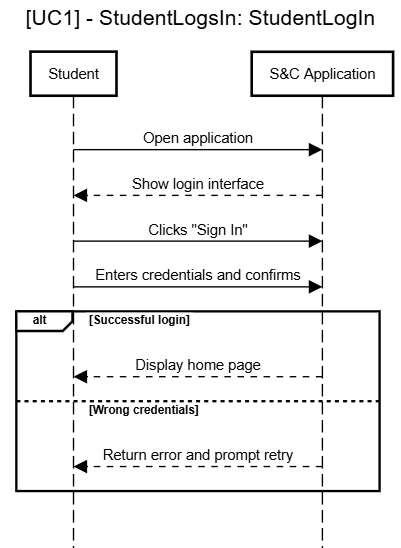
\includegraphics [width=.7\linewidth] {UC1.png}
    \caption{Student Login}
\end{figure}

\begin{figure} [H]
    \centering
    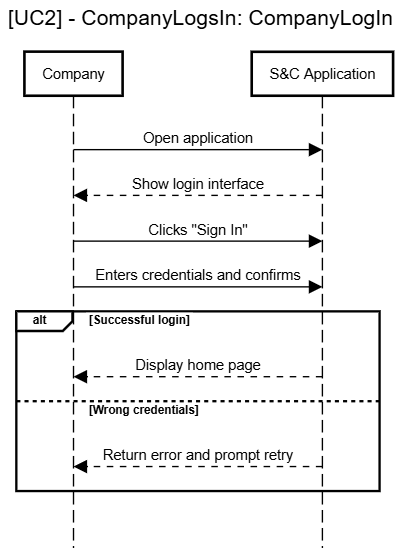
\includegraphics [width=.7\linewidth] {UC2.png}
    \caption{Company Login}
\end{figure}

\begin{figure} [H]
    \centering
    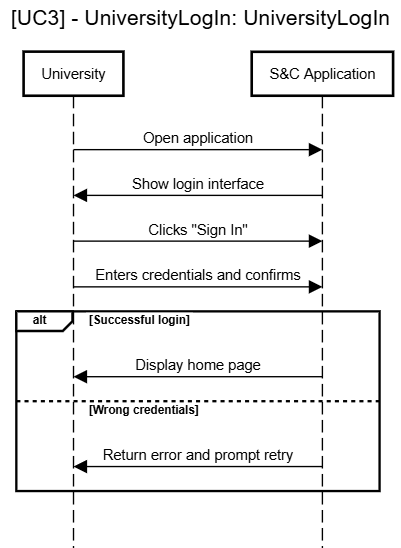
\includegraphics [width=.7\linewidth] {UC3.png}
    \caption{University Login}
\end{figure}

\begin{figure} [H]
    \centering
    
    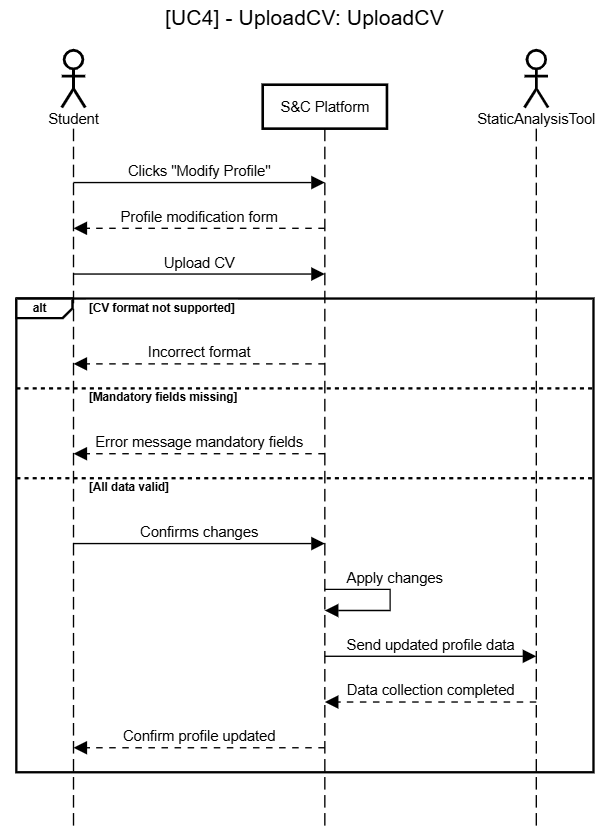
\includegraphics [width=.7\linewidth] {UC4.png}
    \caption{Upload CV}
\end{figure}

\begin{figure} [H]
    \centering
    
    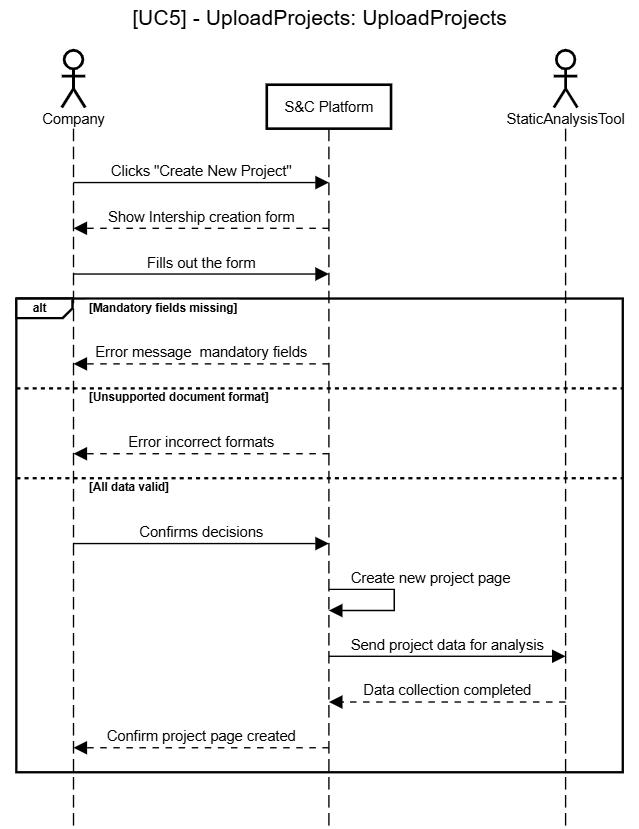
\includegraphics [width=.7\linewidth] {UC5.png}
    \caption{Upload Projects}
\end{figure}

\begin{figure} [H]
    \centering
    
    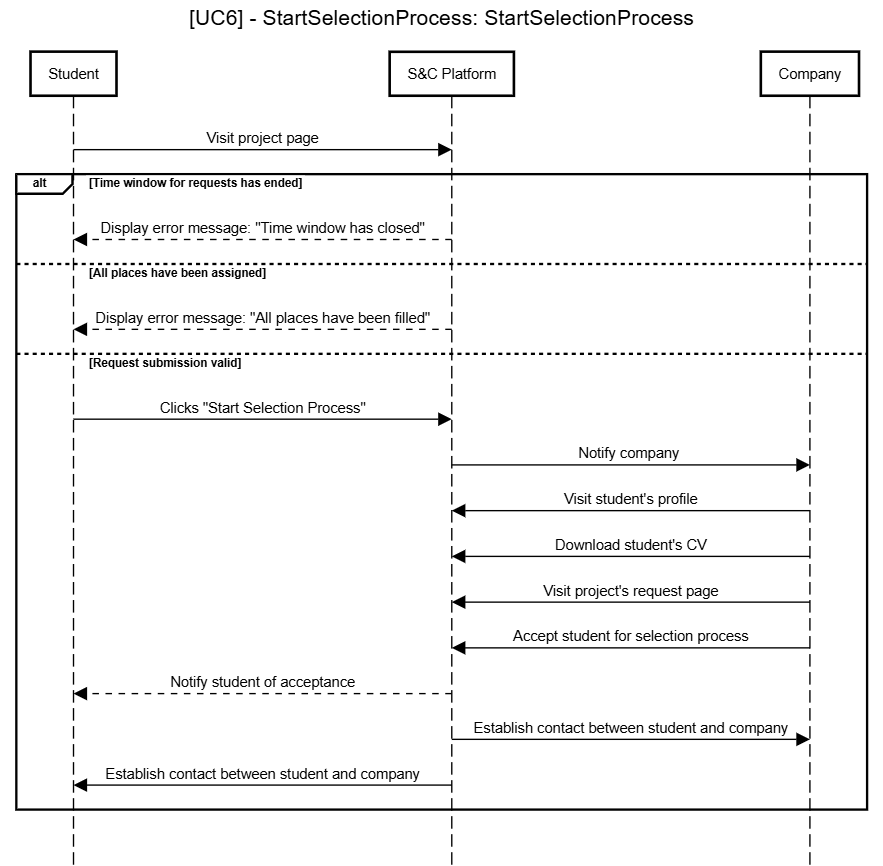
\includegraphics [width=.7\linewidth] {UC6.png}
    \caption{Start Selection Process}
\end{figure}

\begin{figure} [H]
    \centering
    
    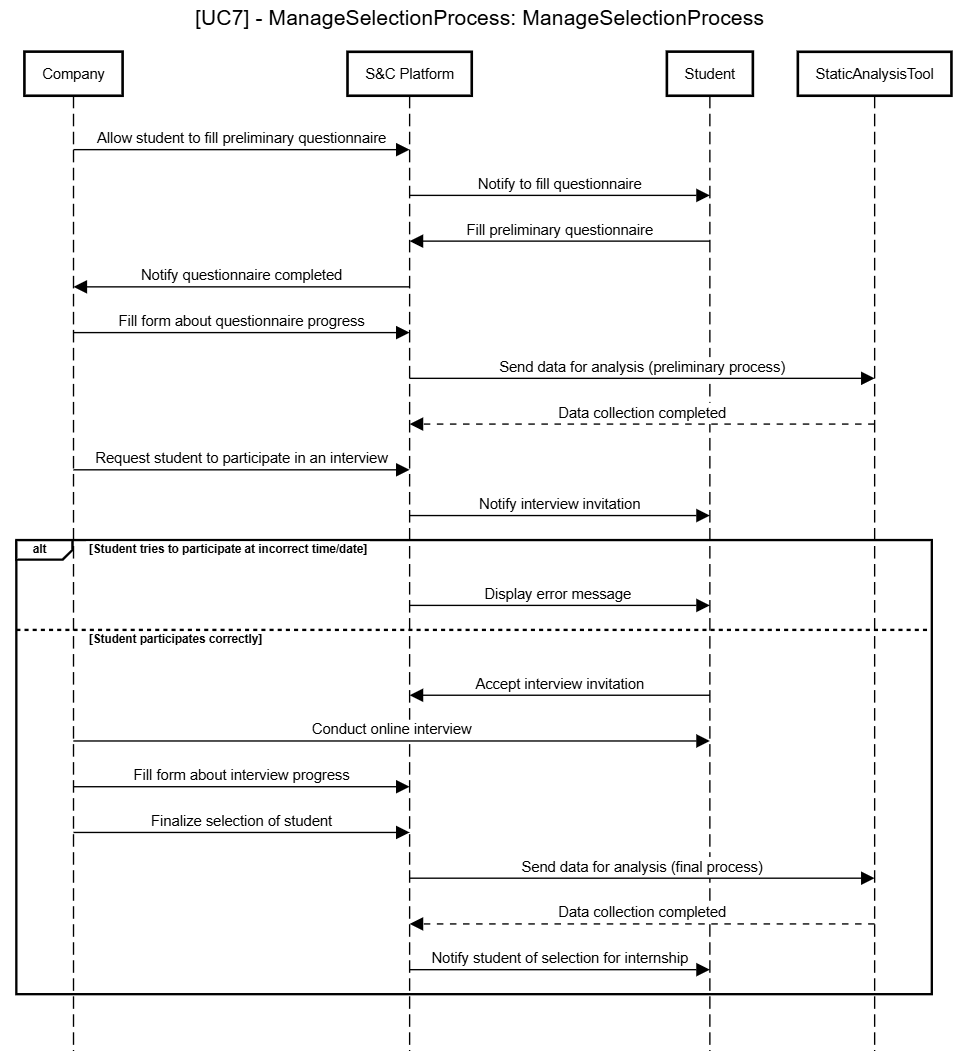
\includegraphics [width=.7\linewidth] {UC7.png}
    \caption{Manage Selection Process}
\end{figure}

\begin{figure} [H]
    \centering
    
    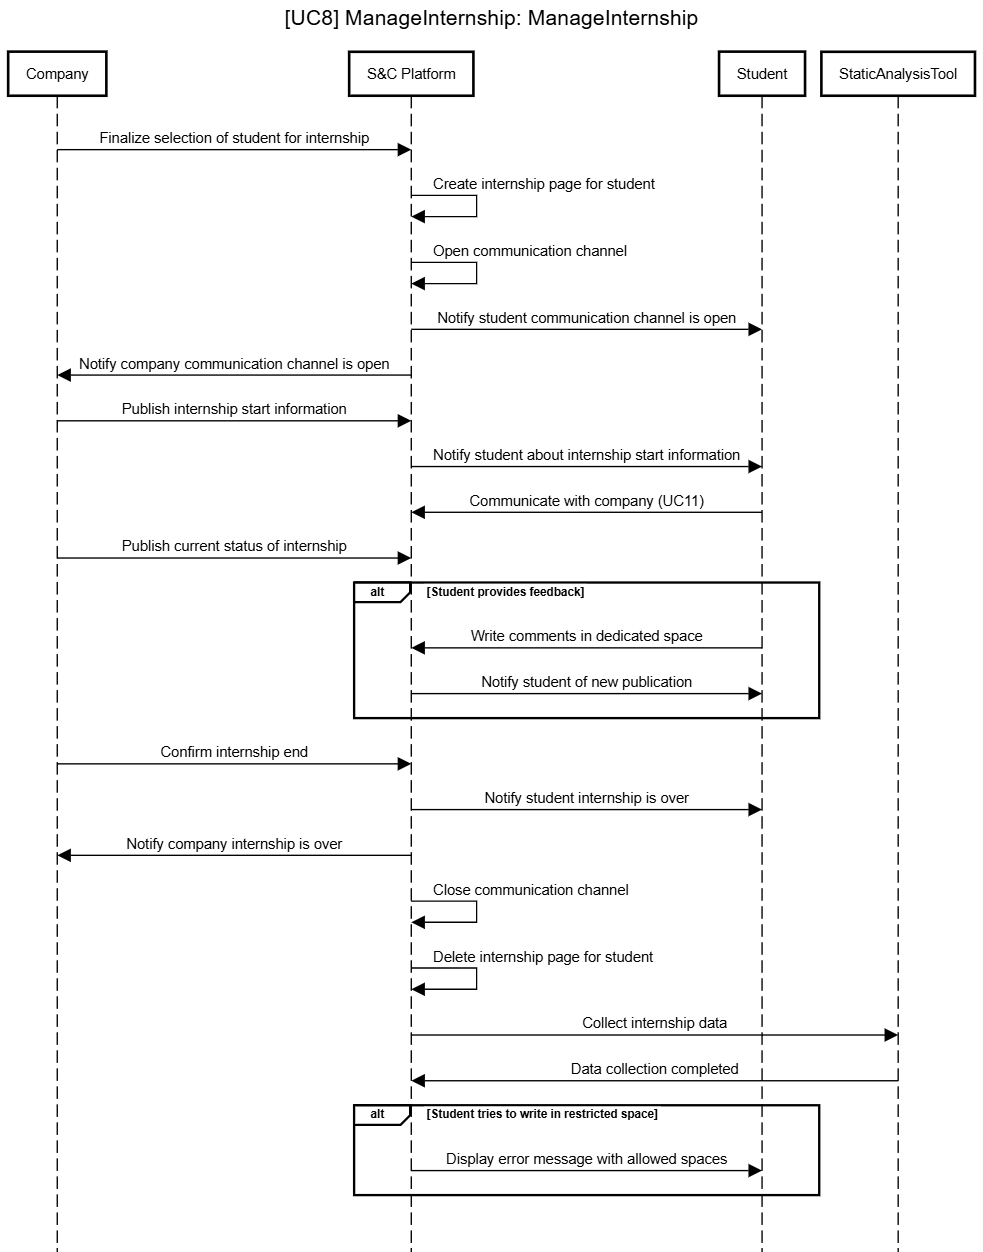
\includegraphics [width=.7\linewidth] {UC8.png}
    \caption{Manage Internship}
\end{figure}

\begin{figure} [H]
    \centering
    
    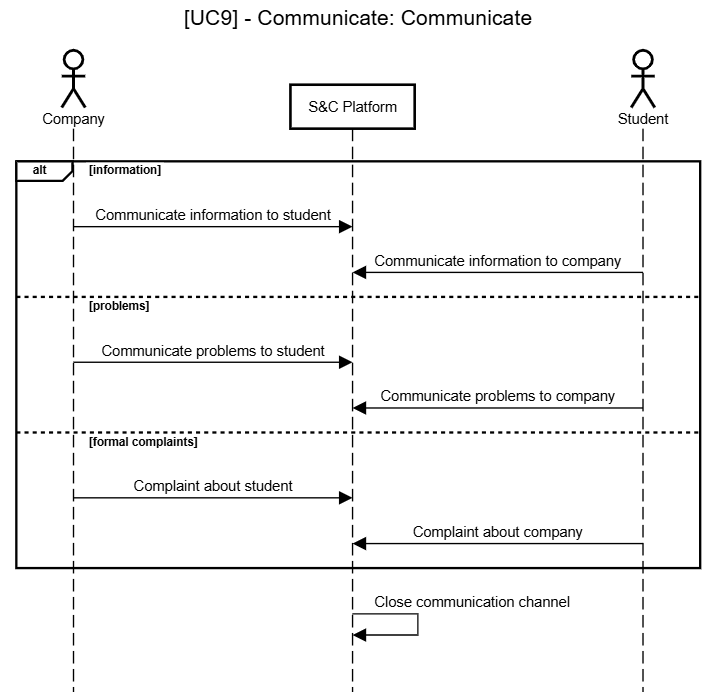
\includegraphics [width=.7\linewidth] {UC9.png}
    \caption{Communicate}
\end{figure}

\begin{figure} [H]
    \centering
    
    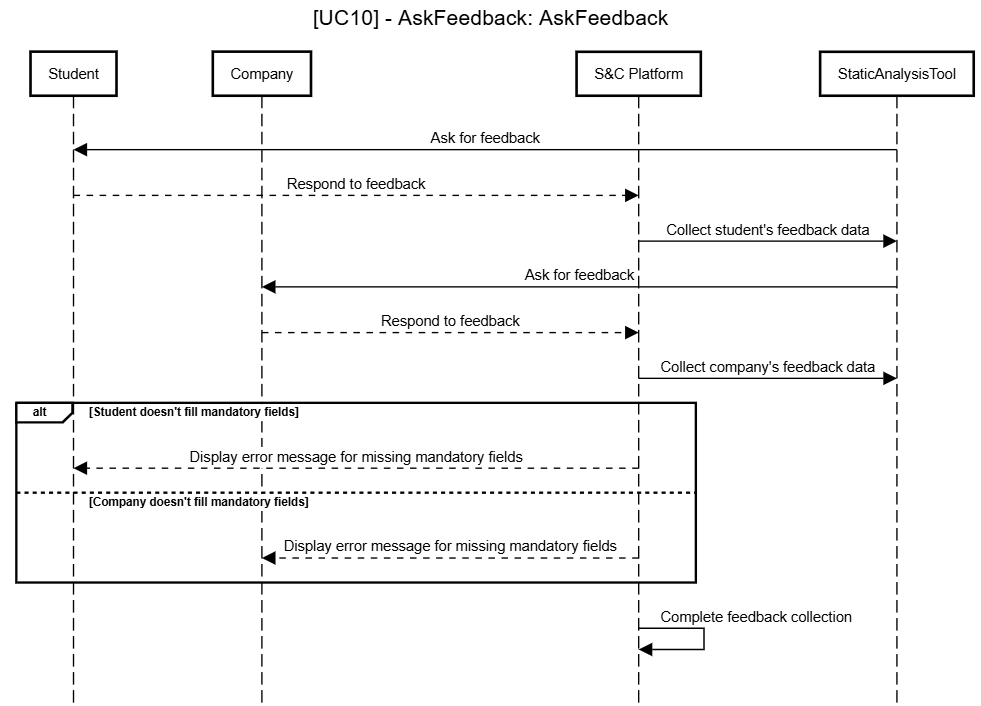
\includegraphics [width=.7\linewidth] {UC10.png}
    \caption{Ask Feedback}
\end{figure}

\begin{figure} [H]
    \centering
    
    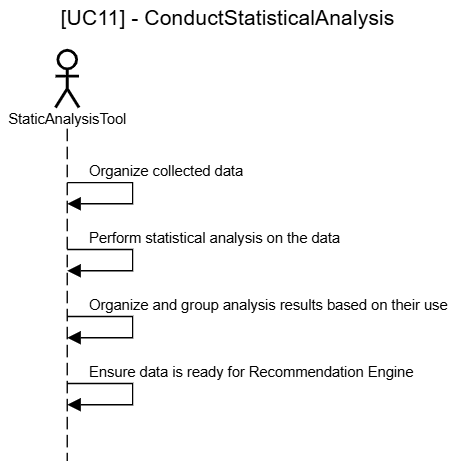
\includegraphics [width=.7\linewidth] {UC11.png}
    \caption{Conduct Statistical Analysis}
\end{figure}

\begin{figure} [H]
    \centering
    
    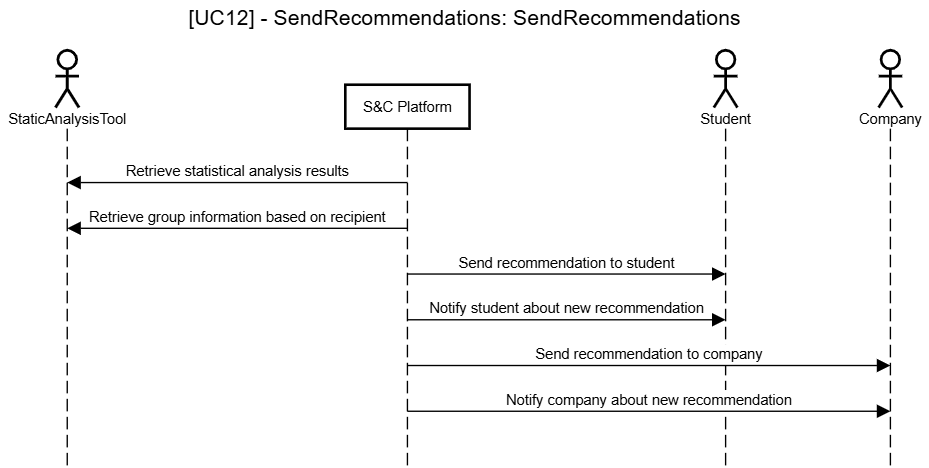
\includegraphics [width=.7\linewidth] {UC12.png}
    \caption{Send Reccommendations}
\end{figure}

\begin{figure} [H]
    \centering
    
    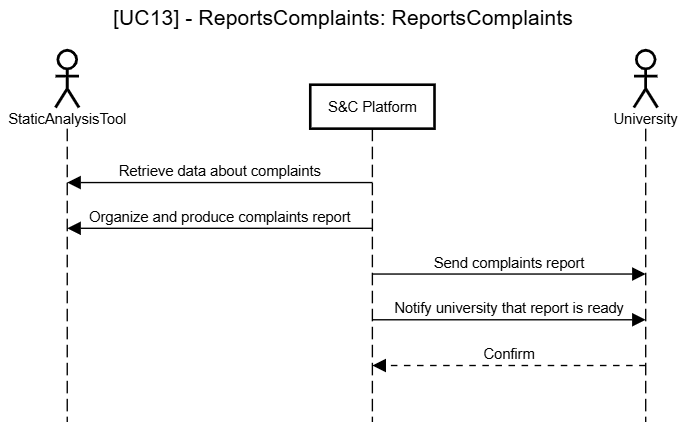
\includegraphics [width=.7\linewidth] {UC13.png}
    \caption{Reports Complaints}
\end{figure}

\begin{figure} [H]
    \centering
    
    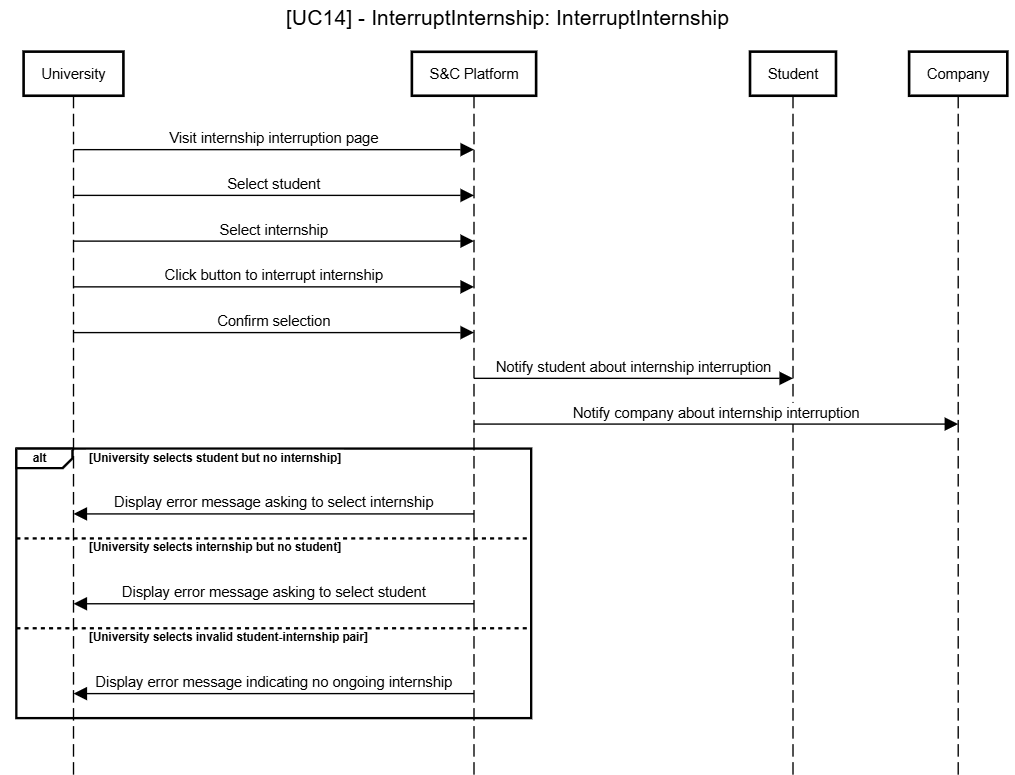
\includegraphics [width=.7\linewidth] {UC14.png}
    \caption{Interrupt Internship}
\end{figure}


\subsection{Activity Diagrams}

\newpage
\subsection{Requirements Mapping}

This table shows a mapping between:
\hspace*{15mm}
\begin{itemize}
    \item Requirements, presented in section 2.2.1.
    \item Goals, presented in section 1.1.
    \item Use Cases, presented in section 3.2.2.
    \item Sequence Diagrams, presented in section 3.2.3
\end{itemize}
\hspace*{15mm}


\begin{longtable}{cccc}
    
    \toprule
    \textbf{Requirement} & \textbf{Goal} & \textbf{UseCase} & \textbf{SequenceDiagram} \\
    \midrule
    \endfirsthead
    
    \toprule
    \textbf{Requirement} & \textbf{Goal} & \textbf{UseCase} & \textbf{SequenceDiagram} \\
    \midrule
    \endhead
    
    \bottomrule
    \endfoot
    
    R1.1 & G1 & UC1    & SD1  \\
    R1.2 & G1 & UC4    & SD4  \\
    R1.3 & G1 & UC4    & SD4  \\
    R1.4 & G1 & UC6  & SD6 \\
    R2.1 & G2 & UC2    & SD2  \\
    R2.2 & G2 & UC5    & SD5  \\
    R2.3 & G2 & UC5  & SD5 \\
    R3.1 & G3 & UC12  & SD12 \\
    R3.2 & G3 & UC6 & SD6 \\
    R3.3 & G3 & UC4-5  & SD4-5 \\
    R3.4 & G3 & UC12  & SD12 \\
    R3.5 & G3 & UC11  & SD11 \\
    R3.6 & G3 & UC7   & SD7  \\
    R3.7 & G3 & UC8    & SD8  \\
    R3.8 & G3 & UC10    & SD10  \\
    R4.1 & G4 & UC6  & SD6 \\
    R4.2 & G4 & UC6 & SD6 \\
    R4.3 & G4 & UC7  & SD7 \\
    R4.4 & G4 & UC7  & SD7 \\
    R4.5 & G4 & UC7  & SD7 \\
    R5.1 & G5 & UC8    & SD8  \\
    R5.2 & G5 & UC9    & SD9  \\
    R6.1 & G6 & UC3    & SD3  \\
    R6.2 & G6 & UC13  & SD13 \\
    R6.3 & G6 & UC14 & SD14 \\


    \end{longtable}

    
\section{Performance Requirements}
The S\&C Platform must meet the efficiency standards for all users. 
The system should be optimized for high performance, with an emphasis on low latency and fast processing speed. 
Response times must not exceed a few seconds under typical operating conditions.
 Additionally, the system should prioritize accuracy in data delivery, as a significant portion of users will be professionals in their respective fields.

\section{Design Constraints}

\subsection{Standard Compliance}
The S\&C Platform must follow the industry standards 
and the best practices to ensure security and scalability. 
These include, but are not limited to, 
data protection regulations such as GDPR (General Data Protection Regulation) 
for safeguarding user data, in addition to all the different national regulations regarding privicy and security.
Additionally, the platform should comply with the IEEE standards 
for software development processes.

\subsection{Hardware Limitations}
The S\&C Platform is designed to operate on standard
 web servers with configurations capable of handling a high volume of concurrent users. 
 While specific hardware requirements will vary depending on deployment scale, 
 the platform should be able to run efficiently on typical cloud infrastructure, 
 such as AWS, Microsoft Azure, or Google Cloud, with adequate CPU, memory, and storage capacity. 
 The system architecture must be flexible to scale horizontally in order to accommodate very dynamic traffic loads without lowering the performance.

\subsection{Other Constraints}
Other constraints affecting the design of the S\&C Platform include:
\begin {itemize}
\item Browser Compatibility: The system must support major web browsers, 
including Chrome, Firefox, Edge, and Safari, with full functionality 
available on both desktop and mobile platforms.
  
\item User Privacy and Security: The platform must ensure that all user data, 
including sensitive information such as CVs and personal profiles, 
is encrypted both in transit and at rest.
  
\item Internationalization and Localization: The platform should be designed 
to support multiple languages and regional settings, allowing accessibility
based on every geographical areas served by the platform.
\end {itemize}
\section{Software System Attributes}

\subsection{Reliability}
The S\&C Platform must be designed for high reliability, 
ensuring that the system operates without failure under normal usage conditions. 
The System should be capable of handling errors gracefully and maintaining stable performance even during peak load scenarios. 
The platform should provide a consistent user experience avoiding unnecessary failures, 
monitoring tools will be implemented to detect issues and allow for quick responses to any system failures.

\subsection{Availability}
The S\&C Platform must be highly available, 
minimizing downtime and maximizing uptime. 
The system architecture will include automated backups and recovery procedures to protect users' data 
and allow for quick restoration in case of failure. 
The system is aiming for an uptime goal of 99.9\% or higher.

\subsection{Security}
Security is a top priority for the S\&C Platform, 
given the sensitive nature of user data (e.g., CVs, personal information, passwords and emails). 
The platform will implement strong encryption (e.g., AES-256) 
for both data at rest and data in transit. 
Furthermore, the platform will follow secure coding practices 
and conduct regular security audits to identify and address potential vulnerabilities. 
Compliance with data protection regulations, such as GDPR, will also be ensured to safeguard user privacy.

\subsection{Maintainability}
The S\&C Platform will be designed with maintainability in mind, 
ensuring that the system can be easily updated and extended. 
The codebase will follow established software engineering best practices, 
such as modularity, code reusability and design patterns, to allow for easier debugging and bug fixes, 
every aspect of the codebase should be well documented for future developments.  
A rigorous testing routine that covers at least 80\% of the codebase will avoid major risks.

\subsection{Portability}
The S\&C Platform will be built with portability in mind, 
ensuring that it can run across different environments, 
including various operating systems (e.g., Windows, Linux, macOS) and web browsers. 
The platform’s front-end will also be responsive, 
adapting seamlessly to different screen sizes and devices (e.g., desktops, tablets, smartphones).
